\section{Microcontroller}

\subsection{OS}
Det er vigtigt i enhver kode situation, der inkluderer flere tasks, at kunne skifte mellem dem på en fornuftig måde; Dette gøres med en scheduler. Når der skal implementeres en scheduler skal det overvejes hvorvidt det er nødvendigt at lave en designed specielt til projektet, eller om der en en eksisterende der er i stand til at udfører opgaven tilstrækkeligt. I dette project har vi to muligheder til rådighed: FreeRTOS eller RTCS.

\subsubsection{RTCS}


\subsubsection{FreeRTOS}

FreeRTOS er et realtid operativsystem (RTOS), som er en standard løsning som bliver brugt i en mikroprocesser. FreeRTOS giver os muligheden for at bruge preemptiv skedulering, Det vil sige at CPU'en kan sprænge i mellem task og hoppe ud af en task efter behov. Dette bliver styret ud af hvilken prioritet taskén har eller om der en anden task, der for et interrupt den skal holde øje med.
\\
Udover dette har freeRTOS også mange andre funktioner dette projekt kan udnytte. Der er mulighed for at oprette køer, som vil blive nævnt som queues. Disse queues kan man sende events og data til ved hjælp af en funktion der hedder xQueueSend. Hvor der så samtidig med at der en der kan tage noget fra denne queue. 
\\
For at kunne gøre det muligt at flere task's skal kunne til gå disse queue's, dette kan gøres ved at bruge noget det hedder en semafor, som gør at kun en task der har adgang til queue'en indtil semaforen bliver frigjort igen. For at ungå at at styre systemet ikke bliver fastlåst i denne semafor for evigt sætte man en tid, den kan være inde i semaforen.
\\
For at nogle af disse ting kan bliver aktiveret skal der føre oprettes en xQueueHandle og xSemaphoreHandle. Hvorefter de bliver kreeret hved hjælp af xQueueCreate og xSemaphoreCreateMutex. For at bruge xQueueCreate skal der også bruges størrelse af queue'en og hvilken parameter den skal indeholde. 

\subsubsection{RTCS}

Run To Complete Scheduler (RTCS) er en måde at køre ens styresystem på. Den køre som en non preemtiv skedulering, det vil sige at lige så snart CPU'en har forbindelse til en proces/task, så kan den ikke hoppe ud af denne proces/task. I dette system kan der oprettes queue's.
//
Den har mulighed for at oprette semafoere, som gør at det er kun en queue som kan have adgang til queue'en. For at tilføje data til en queue skal funktion put\textunderscore queue. wait\textunderscore sem bruges til at tilføje en semafor til den specifikke queue.

\subsubsection{Del konklusion}

Efter vi har set på disse to valg muligheder kan vi se at RTCS vil være næmmere at få til at virker, men at det heller ikke er lige så sikkert, som freeRTOS. Den største begrundelse for at vi vælger at arbjede med freeRTOS over RTCS er at den køre preemtiv. Dette gøre det muligt vis der kommer et vigtigt interrupt at den kan tage CPU'en fra den proces den er i gang med og flytte den over det den mere vigtige proces.

\subsection{Koordinatoversættelse}

For at overholde modularitets princippet er det besluttet systemet skal benytte polære koordinater. For så at kunne benytte de horizontale koordinater som de objekter vi følger skal der laves en transformation fra det horizontale koordinat rum til det polære koordinat rum.

\subsection{Tasks}

\subsubsection{Uart}

Uart står for universal asynchronous receiver/transmitter. Dette laver kommunikation mellem to enheder. Så være enhed skal være i stand til at bruge funktion UART. UART transmittere data i form af bytes og deler dem op i bits og sender dem. Modtager skal så kunne samle dem sammen igen til bytes for at læse det.
Vores Uart pinde sider på PORT A, derved skal sysctl aktiveres på port a før den viker. Uart har en init. funktion som bliver kaldt en gang hvor alle register bliver sat up som, f.eks. send og modtag. Der bliver også sat en baut rate, som skal være den samme for sender og modtager.
\\
For at sende data kalder vi funktion uart0\textunderscore putc som tager en karakter. Dette kan både være tal og bogstaver. Der en funktion der hedder uart0\textunderscore rx\textunderscore rdy som venter på at den modstager noget.
\\
Uart er en god måde til at sende information når man f.eks. skal debugge eller vil have nogen bestemte data hen til ens computer.

\subsubsection{LCD}

Den fysiske opsætning af LCD'et kan ses på figur \ref{fig:LCD}, og viser blandt andet at fire databen og R/W benet er forbundet til stel. Med denne opsætning kan man kun skrive til displayet ligesom man er tvunget til at bruge LCD'et i 4-bit mode. Hvis man havde mulighed for at læse fra displayet, kunne man holde øje med et busyflag, der fortæller om LCD'et er optaget, og på den måde sørge for at udnytte displayets tid bedst muligt. Når man kun kan skrive til displayet, er man tvunget til at vente en bestemt tid for at sikre sig at det er klar til at modtage ny data. Til de fleste formål er det dog ikke et problem, at man venter lidt længere end nødvendigt imellem kommandoer. I 4-bit mode kan der kun sendes en nibble ad gangen. For at sende data til displayet, skal dataen skrives ud på de fire databen, derefter flasher man E-benet så LCD'et kan latche og starte behandlingen. RS-benet styrer om den data, der sendes, skal tolkes som data eller en kommando. 

\begin{figure}[ht]
			\begin{center}
			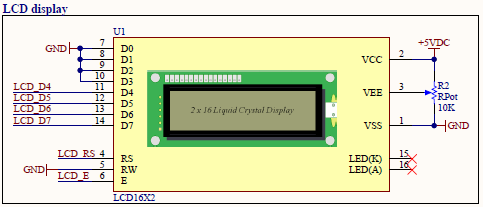
\includegraphics[scale=0.9]{Billeder/LCD.PNG}
			\end{center}
			\caption{LCD pinout}
			\label{fig:LCD}
\end{figure}

Selve LCD-tasken arbejder sammen med resten af systemet ved at afkode et særligt image-format (se figur \ref{fig:LCD_array}), så det vises korrekt på skærmen. Dette image bliver sendt fra display-tasken og indeholder oplysninger om, hvilke karakterer, hvis nogen, der skal skrives til alle 32 synlige adresser på displayet. Udover de 32 karakterer, er der også fire kontrolfelter, som fortæller tasken, hvor cursoren skal placeres efter karaktererne er skrevet ud; om cursoren skal blinke eller bare highlighte nuværende adresse med en streg under karakteren. Det sidste felt bliver sat til at vise adressen, hvor næste karakter skal skrives, når alle 32 karakterer er blevet skrevet første gang. På den måde kan LCD-tasken afgøre om den skal skrive et helt image fra starten, eller bare tilføje en ny karakter til et image der allerede er vist på displayet. Med dette setup kan LCD-tasken finde ud af hvilken ny karakter, der skal tilføjes ud fra den første kontrol-bit, og også hvor cursoren skal placeres efter den er skrevet - hvis den næste adresse, der skal skrives på, er mere end en plads væk, skal cursoren flyttes aktivt. Manipuleringen af images og kontrol-bits foregår i display-tasken - LCD-tasken afkoder bare images, når de bliver tilføjet til dens input-kø.


\begin{figure}[ht]
			\begin{center}
			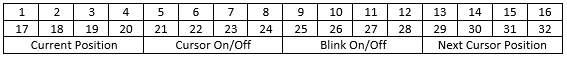
\includegraphics[scale=0.9]{Billeder/LCD_Array.PNG}
			\end{center}
			\caption{LCD Image-format er et array af 36 8-bits størrelser. De første 32 pladser i arrayet repræsenterer de synlige adresser på displayet - de sidste 4 er kontrol-bits.}
			\label{fig:LCD_array}
\end{figure}

\subsubsection{Keypad}

Det udleverede Kit er der tilhørende keypad med 12 knapper fra 0 til 9 og *,\#. Dette keypad virker som knapper, Da er derfor nødvendigt at definere hvad de forskellige knapper skal gøre. For at gøre det simpelt bliver hver knap det som der står på keypad'et. figur \ref{fig:Keypadpins} viser hvordan dens pins at tilsluttet.
\begin{figure}[ht]
	\begin{center}
		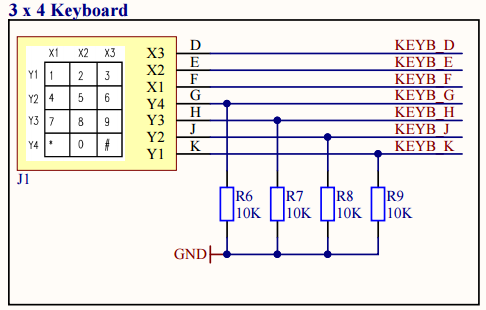
\includegraphics[scale=0.7]{Billeder/Keypadpins.PNG}
	\end{center}
\caption{Keypad pins}
\label{fig:Keypadpins}
\end{figure}
Den har to porte til knyttet som er PORT A og PORT E. Det betyder at vi kan læse på PORT E hvis GPIO pinden på PORT A er aktiv.
\begin{figure}[ht]
	\begin{center}
		\includegraphics[scale=0.7]{Billeder/Keypad.PNG}
	\end{center}
\caption{Keypad struktur}
\label{fig:Keypad}
\end{figure}


På figur \ref{fig:Keypad} kan vi se at vi har givet de forskellige knapper unikke værdier. Dette gøres fordi vi har et array som indeholder alle værdier på keypad’et, som vi så sender ind i bufferen og læse på. For at finde en karakter kigger vi først på alle X værdier (PORT A) igennem og ser om en Y værdi (PORT E) er aktiv og ud fra hvilken X og Y værdi kan vi finde hvilket plads i arrayet ud fra figur \ref{fig:Keypad}
\\
Dette keypad kan blive brugt til at sende data eller manuelt indsætte nogle værdier i mens programmet kører.




\subsection{Serial Peripheral Interface}

Microcontrolleren der blev udleveret dette semester (TM4C123GH6PM) indeholder 4 SSI (Synchronous Serial Interface) da disse 4 interfaces alle er ens, på undtagelse deres pins, er SSI0 blevet valgt som interface, dvs. port A pin 2 er til SSI0Clk (modulets clock), pin 3 er SSI0Fss (frame signalet), pin 4 er SSI0Rx (modtagelse), og pin 5 er SSI0Tx (afsendelse)

Til SSI modulet er der 3 forskellige data formater:

\begin{itemize}
	\item Texas Instruments Synchronous Serial
		\begin{figure}[ht]
			\begin{center}
			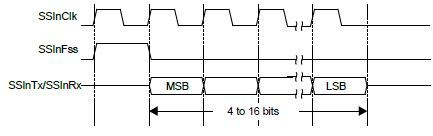
\includegraphics[scale=1]{Billeder/TI_Synchronous_Serial_Frame_Format.jpg}
			\end{center}
			\label{fig:TIFrameFormat}
			\caption{TI Synchronous Serial Frame Format (Single transfer)}
		\end{figure}

	\item Freescale SPI
		\begin{figure}[ht]
			\begin{center}
			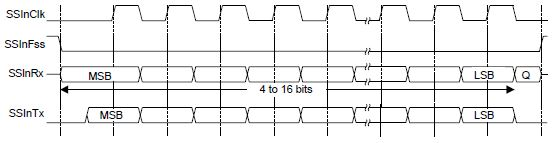
\includegraphics[scale=1]{Billeder/FS_Frame_Format.jpg}
			\end{center}
			\label{fig:FSFrameFormat}
			\caption{FreeScale Frame Format (Single Transfer)}
		\end{figure}
		  
	\item Microwire
		\begin{figure}[ht]
			\begin{center}
			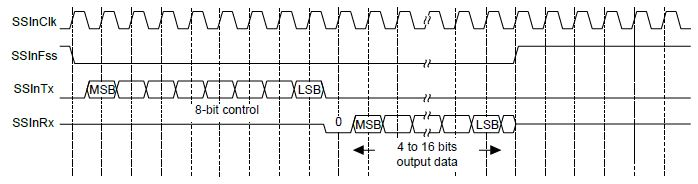
\includegraphics[scale=0.8]{Billeder/MW_Frame_format.jpg}
			\end{center}
			\label{fig:MWFrameFormat}
			\caption{Micro Wire Frame Format (Single Transfer)}
		\end{figure}
\end{itemize}

Da Freescale er den eneste SPI iblandt de tre SSI moduler er det den der blev valgt.

		\begin{figure}[ht]
			\begin{center}
			\includegraphics[scale=0.8]{Billeder/Spi_Setup.jpg}
			\end{center}
			\label{fig:SPI_Setup}
			\caption{Setup af Freescale SPI}
		\end{figure}

For at lave et Freescale setup skal SSI modulet deaktiveres, også kan microcontrolleren sættes som master ved at skrive nul til control registret.
Derefter skal clock configurations registret sættes til 0 så vi bruger system clocken.
Der ønskes en 2 Mbps clock bruges følgende ligning

\begin{align*}
2*10^6 bps &= \dfrac{16*10^6 Hz}{CPSDVSR * (1 + 0)}\\
CPSDVSR &= \dfrac{16*10^6 Hz}{2*10^6 bps}\\
CPSDVSR &= 8
\end{align*}

Så sættes kontrol registret for SSI0 til 0xF da bit 3:0 angiver data størrelse, 0xF er så 16-bit data. Samtidig bliver Freescale SPI sat op, da bit 4 og 5 bestemmer frame formatet, og hvis de begge er lave betyder det at Freescale er valgt. 
og igen sættes bit 1 i kontrol registret for SSI1 til høj så SSI'en er aktiveret.
